\chapter{LitQEval}\label{ch:ownApproach}
Despite ongoing research on automatic literature query generation and related evaluations with medical datasets, such as CLEF \autocite{kanoulas2017clef, kanoulas2018clef, kanoulas2019clef} and the Collection of Seeds \autocite{Wang_2022}, the insights gained from these evaluation metrics are not particularly compelling for our use case. This limitation arises from two main factors. 

First, the CLEF and Collection of Seeds datasets are exclusively focused on medical data. Although Badami's work \autocite{badami2023adaptive} offers a more diverse dataset, it lacks a suitable evaluation metric. Their evaluation primarily aims to maximize recall, with minimal consideration for precision, as literature search queries often yield far more results than necessary, making precision a less effective measure in this context. 

A second limitation arises when recall is prioritized exclusively. For example, if we aim to train a model to generate queries that maximize recall, there is no penalty for generating overly broad queries, such as those that exploit wildcards, which could lead to an excessive number of irrelevant results.

To address these issues, we introduce a dataset structured similarly to that of Badami \autocite{badami2023adaptive} but designed to be more comprehensive and covering a wider range of topics. Alongside this dataset, we propose new evaluation metrics that account for the inherently broad nature of literature search queries while penalizing excessively large queries. These metrics also emphasize the importance of accurately identifying core publications that are deemed highly relevant within the domain.


\section{Dataset}
The dataset we aim to create has two primary goals: First, it should encompass a wide range of randomly selected scientific research fields. Second, for each selected field, it should contain a set of highly relevant publications to serve as anchors for evaluating additional publications found in these areas.

Selecting new research topics is straightforward; however, to avoid bias from ongoing research interests, we used ChatGPT to generate a list of scientific fields that are recent and not overly broad. For instance, a topic like \textit{Artificial Intelligence} is vast, making it challenging to accurately and comprehensively identify core publications. Instead, we chose a more specific, problem-focused topics such as \textit{Drones in Agriculture}. To search for the corresponding bibliometric analysis we used the following query: \textit{<TERM>  ("Bibliometric" OR "Scientometric" OR "Systematic literature" OR "Most Influential" OR "Most Cited" OR "Scientific Landscape" OR "Literature Landscape" OR "Core Literature")} 


After identifying a sufficient number of diverse fields, 15 in our case, we sought to collect core publications for each field. Due to the difficulty of gathering core publications across a broad array of topics, we leveraged the bibliometrics community’s expertise. Specifically, we searched for bibliometric studies that identify the most relevant publications within each research area. For example, a bibliometric analysis of \textit{Drones in Agriculture} \autocite{Rejeb2022} lists the most cited publications from 1990 to 2021. In this case, 40 core publications were identified, which we manually located on Dimensions.ai and added to our dataset, omitting any publications not found in Dimensions.

This process was repeated across all selected research fields, resulting in a dataset containing 15 topics, each with 25–50 core publications, as illustrated in \autoref{fig:dataset-overview}.
\begin{figure}
	\centering	
	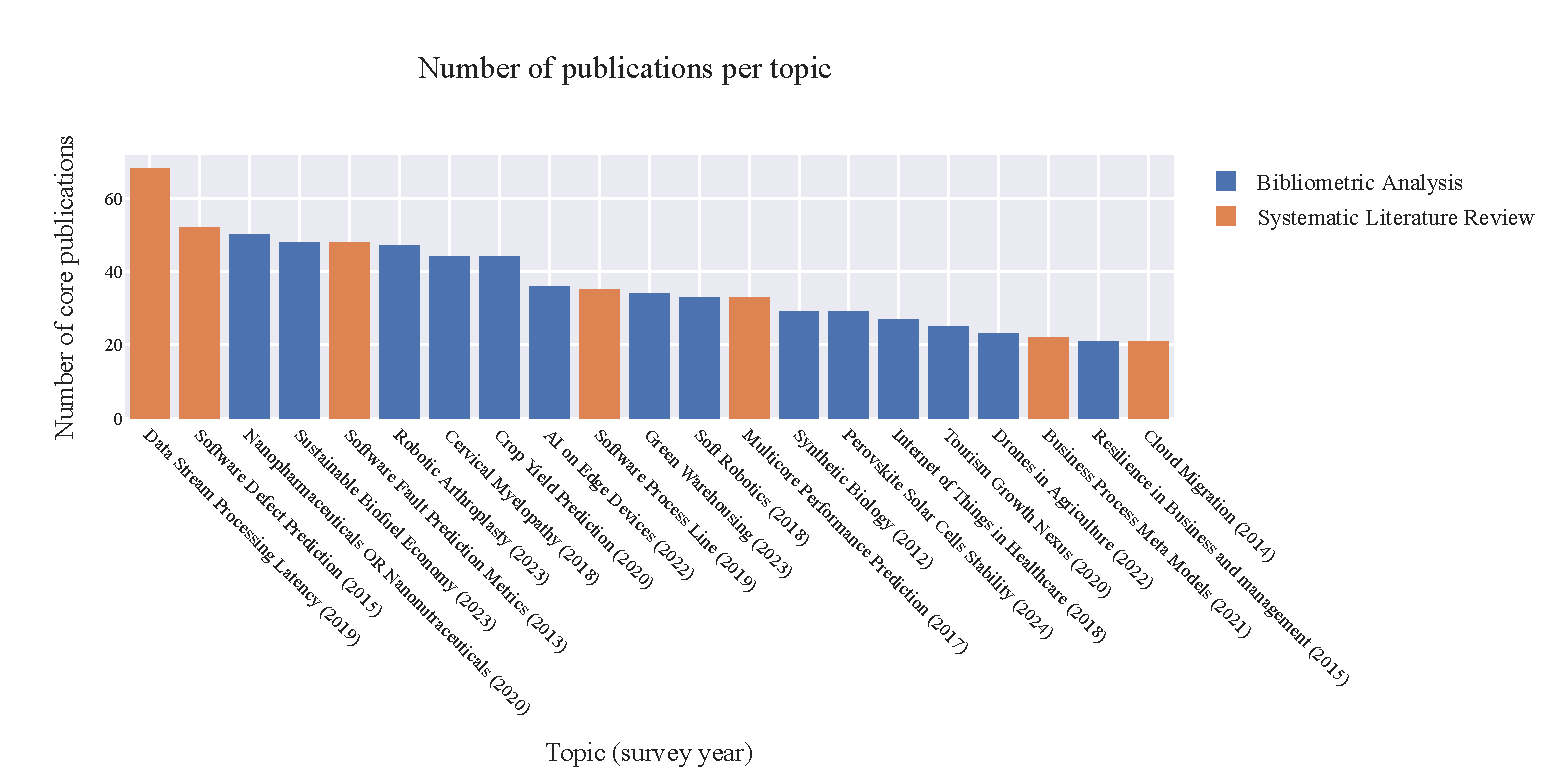
\includegraphics{pics/dataset-overview.pdf}
	\caption[Dataset overview of the research topics]{An overview of the dataset and the selected 15 research fields with respective core publications identified through bibliometric analyses. The number in brackets following the field name on the x-axis represents the year of the analysis.}
	\label{fig:dataset-overview}
\end{figure}


\subsection{Dataset Analysis}
We recognize that potential biases may exist in our dataset due to its complete reliance on the bibliometric community for identifying core publications. This often implies that publications with higher citation counts are deemed more relevant. To assess this, we analyzed the citation distribution per topic, as provided by Dimensions, shown in \autoref{fig:dataset-citation}. Additionally, we examined the distribution of publication years per topic, illustrating the time span considered in the bibliometric analyses, as shown in \autoref{fig:dataset-years}.  If we compare the distribution of publication years for the medical research field \textit{Cervical Myelopathy} with that of \textit{IoT in Healthcare}, both of which were published in 2018, we can observe distinct differences in the year distributions of their core publications. These variations may be attributed to factors such as the recency of the field, changes in terminology over time, or the nature of the research area, where one field may prioritize more established works while the other focuses on recent advancements.

\begin{figure}
	\centering	
	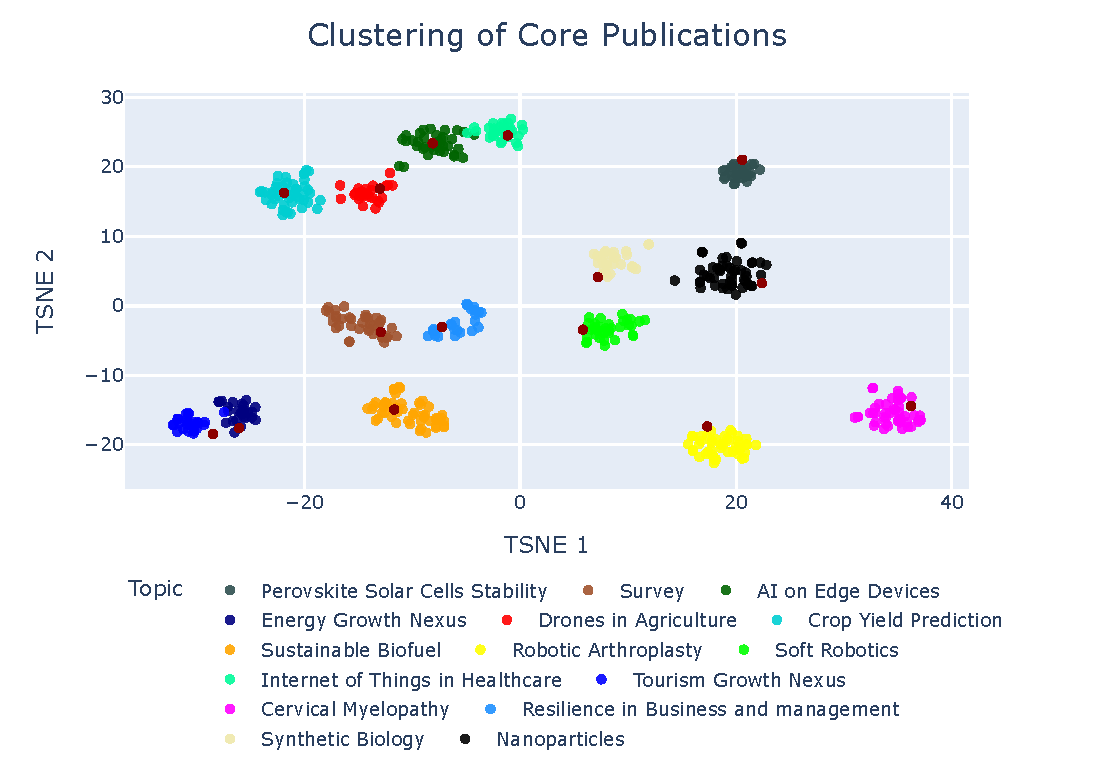
\includegraphics[scale=0.4, width=350px]{pics/tnse_clustering.pdf}
	\caption[Core Publications Clustering]{This figure shows clusters of publication embeddings based on titles and abstracts. Embeddings were generated with OpenAI's small model and reduced in dimensionality with t-SNE, then clustered using k-means with $k=15$ (indicating topic count). Clusters group core publications by semantic similarity, with overlaps in topics like \textit{IoT in Healthcare} and \textit{AI on Edge Devices}, as well as \textit{Tourism Growth Nexus} and \textit{Energy Growth Nexus}, due to the similarity in the research field.}
	\label{fig:dataset-clustering}
\end{figure}

For the evaluation pipeline that we will introduce, the embeddings of the core documents are essential for effectively assessing the search query, as detailed in \autoref{sec:eval-metrics}. To validate this approach, we examine the clustered embeddings of the titles and abstracts for each core topic, as well as the bibliometric analyses in which these documents were initially referenced. This enables us to assess whether core publications within each field exhibit semantic similarity while also demonstrating some degree of dissimilarity from publications in other topics. The resulting clusters, shown in \autoref{fig:dataset-clustering}, were generated using k-means clustering, where $k$ is set to the number of topics. For this, we use OpenAI's small embeddings model alongside t-SNE\autocite{van2008visualizing} to reduce the dimensionality to 2D.


\section{Evaluation metrics}\label{sec:eval-metrics}
The standard evaluation metrics for query evaluation are recall and precision. We argue that while recall is of high importance, particularly within the community, precision in this context becomes less feasible. Specifically, retrieving only the exact core publications via a search query would be impractical without explicitly using DOIs to target them directly, which renders this metric largely obsolete and likely to be consistently low. However, we still aim to account for the number of matched publications when executing a search query to prevent models from exploiting overly large queries. To address this, we introduce the concept of \textit{Semantic Precision}.

The idea behind Semantic Precision is to evaluate the relevance of retrieved publications in comparison to the core publication set. If the retrieved publications are sufficiently similar to those in the core set, they are deemed to hold some relevance rather than being entirely unrelated. To achieve this, we propose that the core publications, encompass sufficient semantic breadth to gauge the quality of literature relevant to a specific field. We calculate Semantic Precision in two ways.

\begin{figure}[h!]
	\centering	
	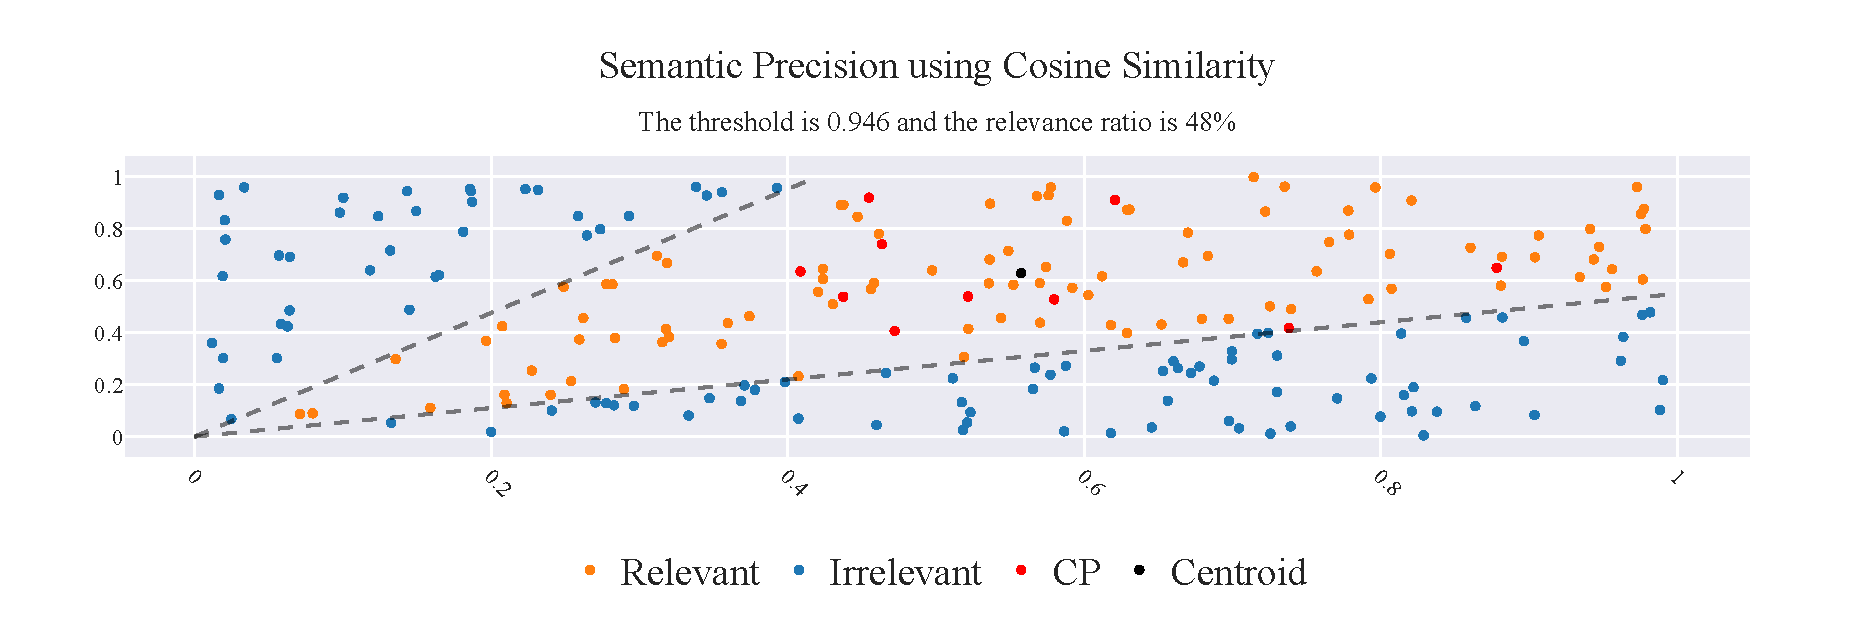
\includegraphics[scale=0.4]{pics/sp_cos.pdf}
	\caption[Semantic Precision using Cosine Similarity]{This illustration demonstrates the effect of cosine similarity on randomly generated data in a 2D space. The core publications (CP) are shown in red, positioned between 0.4 and 0.9 on both the x- and y-axes. When we set the threshold to 0.946, based on the cosine similarity of the least similar core publication from the centroid, many retrieved publications on the opposite side of the spectrum are still assigned as relevant. This effect occurs because cosine similarity considers only the angle between vectors, ignoring their magnitude. In this case, this results in 48\% of the retrieved publications being considered relevant.}

	\label{fig:sp-cos}
\end{figure}


The first approach involves averaging the embeddings of the core publications. We then set an acceptance threshold based on the cosine similarity to the least similar core publication, given by. This means that if the embedding of a retrieved publication is more similar to the center than the least similar core publication, we consider it a relevant publication, as shown in \autoref{fig:sp-cos}. We define:
\begin{itemize}
	\item $CPs$ as the set of core publications.
	\item $\vec{c_i}$ as the embedding vector of the $i$-th core publication.
	\item $\vec{p}$ as the embedding vector of a retrieved publication.
	\item $\cos(\vec{a}, \vec{b})$ as the cosine similarity between two vectors $\vec{a}$ and $\vec{b}$.
\end{itemize}

First, compute the centroid of the core publication embeddings:
\[
\vec{c}_{\text{centroid}} = \frac{1}{|CPs|} \sum_{\vec{c_i} \in CPs} \vec{c_i}
\]
Then, let the threshold similarity, $\theta$, be the cosine similarity of the least similar core publication to the centroid:
\[
\theta = \min_{\vec{c_i} \in CP} \cos(\vec{c}_{\text{centroid}}, \vec{c_i})
\]
Finally, Semantic Precision using cosine similarity ($SP_{cos}$) is defined as \autoref{eq:sp-cosine}, where $\mathbb{I}$ is an indicator function that equals 1 if the retrieved publication $\vec{r}$ meets the similarity criterion and 0 otherwise:
\begin{equation}\label{eq:sp-cosine}
	SP_{cos} = \frac{\sum_{\vec{p} \in \text{pubs}} \mathbb{I} \left( \cos(\vec{c}_{\text{centroid}}, \vec{p}) \geq \theta \right)}{|\text{retrieved}|}
\end{equation}

\begin{figure}[h!]
	\centering	
	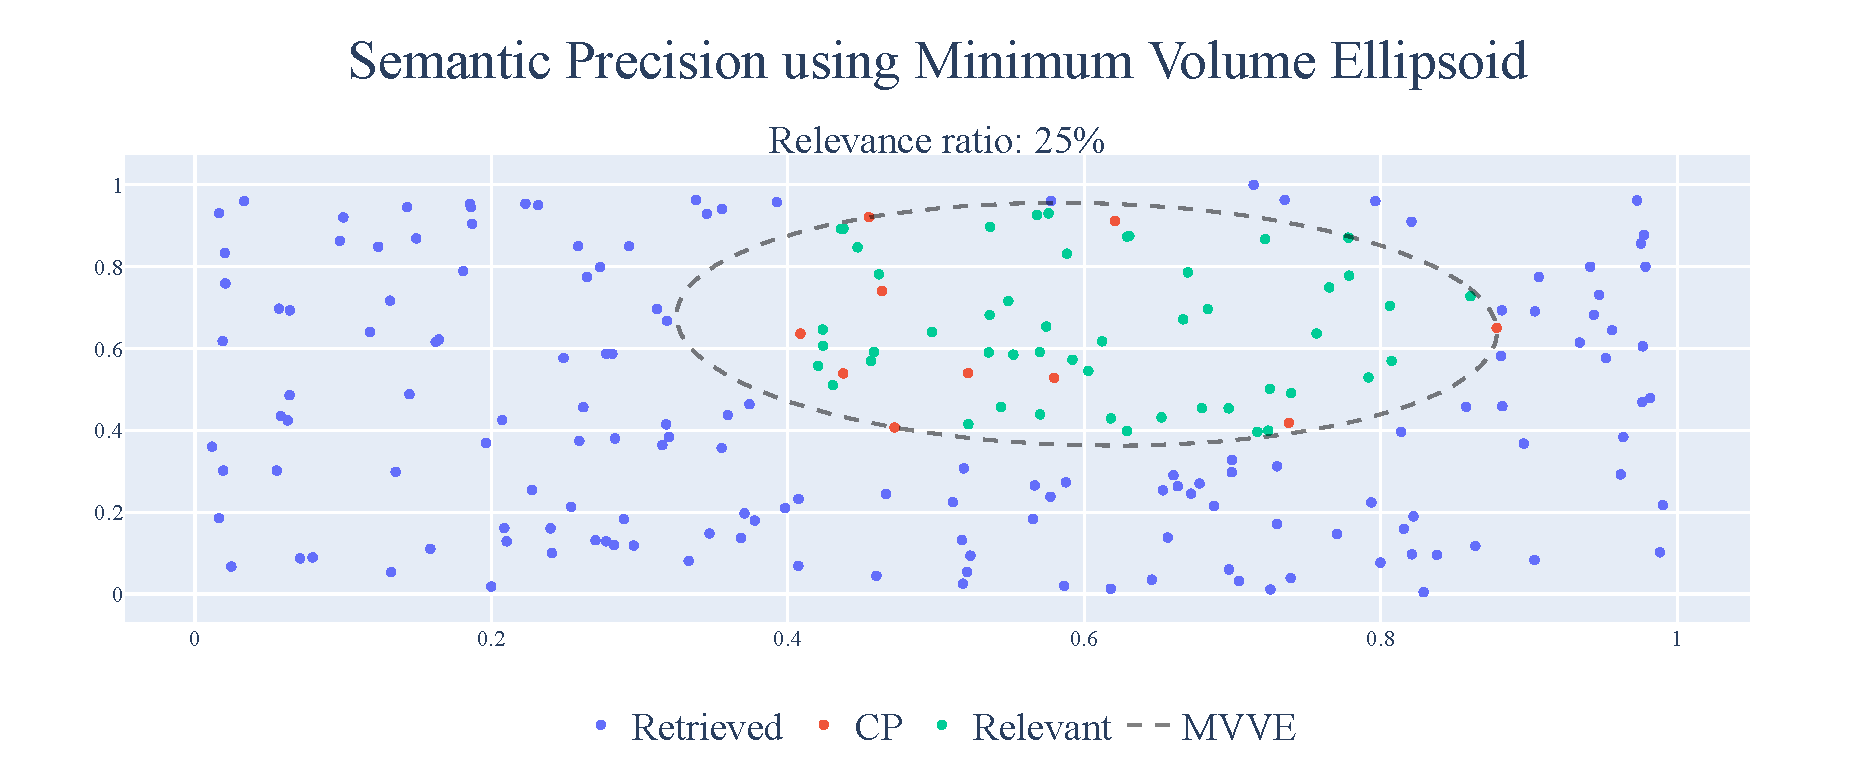
\includegraphics[scale=0.4]{pics/sp_mvee.pdf}
	\caption[Semantic Precision using MVEEE]{This illustration demonstrates the effect of using the Minimum Volume Enclosing Ellipsoid (MVEE) on randomly generated data in a 2D space. The core publications (CP) are shown in red, positioned between 0.4 and 0.9 on both the x- and y-axes. An ellipsoid is generated using MVEE to define the scope of relevant publications, ensuring that only those within the maximal angles and magnitudes of the core publications are considered relevant. In this case, this approach results in only 25\% of the retrieved publications being classified as relevant.}

	\label{fig:sp-mvee}
\end{figure}

For the second approach we omit the averaging of the embeddings and use Minimum Volume Enclosing Ellipsoid (MMVE), which creates the smallest ellipsoid that includes the our CP, which we then use to determine which of the retrieved publications are relevant by checking whether they are within MMVE or not, as illustrated in \autoref{fig:sp-mvee}. This approach allows us to take into account all the dimensions by not only considering the angle but also the magnitude

The Minimum Volume Enclosing Ellipsoid (MVEE) for the core publication set $CP$ is centered at $\delta$ with shape matrix $A$. To determine whether a retrieved publication $\vec{r}$ is relevant, we check if it lies within the ellipsoid by testing the following condition:
\[
(\vec{p} - \delta)^T A (\vec{p} - \delta) \leq 1
\]
Semantic Precision (SP) for this approach is then:

\begin{equation}\label{eq:sp-mvee}
	\text{SP}_{\text{MVEE}} = \frac{\sum_{\vec{p} \in \text{pubs}} \mathbb{I} \left( (\vec{p} - \delta)^T A (\vec{p} - \delta) \leq 1 \right)}{|\text{pubs}|}
\end{equation}

Now that we have a metric that can be used punish the model in case of generating a too broad of a query, we use can use it as a factor to calculate the F-Score, the goal of the standard F-score is to balance out between the recall and precision, but in our case we use $F-\beta$ instead, whereby the $\beta$ is the weighting factor of the recall, meaning the higher it is the more important the recall will be, in our case we set it to be 2, meaning that the recall is twice as important as the precision.
\begin{equation}\label{eq:f-beta}
F_\beta = (1 + \beta^2) \cdot \frac{\text{Precision} \cdot \text{Recall}}{(\beta^2 \cdot \text{Precision}) + \text{Recall}}
\end{equation}
For our specific case where $\beta = 2$, emphasizing the importance of recall, it is:
\[
	F_2 = 5 \cdot \frac{\text{Precision} \cdot \text{Recall}}{(4 \cdot \text{Precision}) + \text{Recall}}
\]

